\chapter{Верификация и примеры расчетов}
\label{ch:verification}

Сравнение численного алгоритма, описанного выше, с МКЭ на задаче статического раскрытия трещины было показано в работе \cite{Peirce2001UniformAA}. В ней показана сопоставимость расчетов данных методов.

Чтобы продемонстрировать влияние неоднородности модулей упругости рассмотрим пласт, состоящий из трех слоев. Толщина внутреннего слоя $20$ м. Рассмотрим модель распространения трещины с равномерной закачкой жидкости в центре внутреннего слоя на протяжение всего процесса. Начальный момент времени $t = 0$~c., конечный $t = 300$~с., утечки жидкости в пласт отсутствуют. $E_i$, $\nu_i$, где $i=\text{b, m, t}$ -- упругие модули нижнего, среднего и верхнего слоев соответственно. 

В случае, если упругие модули всех слоев одинаковы получается модель радиальной трещины (рисунки \ref{fig:homogeneous-planar}, \ref{fig:homogeneous-slice}).
\begin{figure}[htbp]
    \centering
    \begin{subfigure}[t]{0.4\textwidth}
        \centering
        \caption{Раскрытие трещины.}
        \label{fig:homogeneous-planar}
        \includegraphics[width=\textwidth]{Homogeneous/Figures/1/width_29.pdf}
    \end{subfigure}
    \hfill 
    \begin{subfigure}[t]{0.55\textwidth}
        \centering
        \caption{Раскрытие трещины вдоль оси $Oy$, $x=1.5$~м.}
        \label{fig:homogeneous-slice}
        \includegraphics[width=\textwidth]{Homogeneous/Figures/1/w_y_29.pdf}
    \end{subfigure}
    \caption{Радиальная трещина, $E_\text{b} = E_\text{m} = E_\text{t} = 10$~GPa, $\nu_\text{b} = \nu_\text{m} = \nu_\text{t} = 0.22$.}
    \label{fig:homogeneous}
\end{figure}

Рассмотрим пласт, где модуль Юнга $E_\text{b}$ нижнего слоя выше, чем в верхних. Как видно из рисунков~\ref{fig:heterogeneous-2-layer-planar} и \ref{fig:heterogeneous-2-layer-slice} жесткость нижнего слоя сильно влияет на распространение трещины. Расстояние от верхнего кончика трещины до точки закачки жидкости ГРП больше в два раза, чем расстояние от нижнего кончика трещины.
\begin{figure}[htbp]
    \centering
    \begin{subfigure}[t]{0.4\textwidth}
        \centering
        \caption{Раскрытие трещины.}
        \label{fig:heterogeneous-2-layer-planar}
        \includegraphics[width=\textwidth]{Heterogeneous/Figures/1/width_29.pdf}
    \end{subfigure}
    \hfill 
    \begin{subfigure}[t]{0.55\textwidth}
        \centering
        \caption{Раскрытие трещины вдоль оси $Oy$, $x=1.5$~м.}
        \label{fig:heterogeneous-2-layer-slice}
        \includegraphics[width=\textwidth]{Heterogeneous/Figures/1/w_y_29.pdf}
    \end{subfigure}
    \caption{Пласт с жестким нижним слоем, $E_\text{b} = 50$~GPa, $E_\text{m} = E_\text{t} = 10$~GPa, $\nu_\text{b} = \nu_\text{m} = \nu_\text{t} = 0.22$.}
    \label{fig:heterogeneous-2-layer}
\end{figure}


Стоит заметить, что в отличие от неоднородности по сжимающим напряжениям, неоднородность по модулям упругости не образует барьер для роста трещины. Даже при большой разницы модулей Юнга трещина проникает и растет вдоль жесткого слоя. На рисунке~\ref{fig:heterogeneous-high} показан результат для $k=\frac{E_\text{b}}{E_\text{t}} = 10$. На рисунке~\ref{fig:heterogeneous-3layer} изображен случай, где средний слой ограничен более жесткими. Подобный результат был также показан на модели Pseudo3d в работе~\cite{gu2006}.
\begin{figure}[htbp]
    \centering
    \begin{subfigure}[t]{0.4\textwidth}
        \centering
        \caption{Раскрытие трещины.}
        \label{fig:heterogeneous-high-planar}
        \includegraphics[width=\textwidth]{Heterogeneous/Figures/2/width_29.pdf}
    \end{subfigure}
    \hfill 
    \begin{subfigure}[t]{0.55\textwidth}
        \centering
        \caption{Раскрытие трещины вдоль оси $Oy$, $x=1.5$~м.}
        \label{fig:heterogeneous-high-slice}
        \includegraphics[width=\textwidth]{Heterogeneous/Figures/2/w_y_29.pdf}
    \end{subfigure}
    \caption{Пласт с сильной неоднородностью, $E_\text{b} = 100$~GPa, $E_\text{m} = E_\text{t} = 10$~GPa, $\nu_\text{b} = \nu_\text{m} = \nu_\text{t} = 0.22$.}
    \label{fig:heterogeneous-high}
\end{figure}


\begin{figure}[htbp]
    \centering
    \begin{subfigure}[t]{0.4\textwidth}
        \centering
        \caption{Раскрытие трещины.}
        \label{fig:heterogeneous-3layer-planar}
        \includegraphics[width=\textwidth]{Heterogeneous/Figures/3_3/width_29.pdf}
    \end{subfigure}
    \hfill 
    \begin{subfigure}[t]{0.55\textwidth}
        \centering
        \caption{Раскрытие трещины вдоль оси $Oy$, $x=1.5$~м.}
        \label{fig:heterogeneous-3layer-slice}
        \includegraphics[width=\textwidth]{Heterogeneous/Figures/3_3/w_y_29.pdf}
    \end{subfigure}
    \caption{Пласт с сильной неоднородностью, $E_\text{m} = 10$~GPa, $E_\text{b} = E_\text{t} = 100$~GPa, $\nu_\text{b} = \nu_\text{m} = \nu_\text{t} = 0.22$.}
    \label{fig:heterogeneous-3layer}
\end{figure}


Рассмотрим случай, где также присутствует неоднородность сжимающих напряжений. В верхних слоях $\sigma_{h,\text{m}} = \sigma_{h,\text{t}} = 30.5$~MPa выше, чем в нижнем $\sigma_{h,\text{b}} = 30$~MPa. Из рисунка~\ref{fig:comparison-1} видно, что рост трещины обусловлен ростом в нижнем слое, несмотря на то, что его модуль Юнга $E_\text{b} = 20$~GPa больше, чем в верхних слоях $E_\text{m} = E_\text{t} = 10$~GPa. Подобное поведение роста трещины связано с тем, что эффективное напряжение $p_\text{net} = p - \sigma_h$ -- выше в нижнем слое. На рисунке~\ref{fig:comparison-2} приведен пример, где модуль Юнга $E_\text{b} = 40$~GPa компенсирует высокое эффективное напряжение.

\begin{figure}[htbp]
    \centering
    \begin{subfigure}[t]{0.4\textwidth}
        \centering
        \caption{Раскрытие трещины.}
        \label{fig:comparison-1-planar}
        \includegraphics[width=\textwidth]{Heterogeneous/Figures/3/width_29.pdf}
    \end{subfigure}
    \hfill 
    \begin{subfigure}[t]{0.55\textwidth}
        \centering
        \caption{Раскрытие трещины вдоль оси $Oy$, $x=1.5$~м.}
        \label{fig:comparison-1-slice}
        \includegraphics[width=\textwidth]{Heterogeneous/Figures/3/w_y_29.pdf}
    \end{subfigure}
    \caption{Неоднородный по модулям упругости и сжимающим напряжениям пласт, $E_\text{b} = 20$~GPa, $E_\text{m} = E_\text{t} = 10$~GPa, $\nu_\text{b} = \nu_\text{m} = \nu_\text{t} = 0.22$, $\sigma_{h,\text{b}} = 30$~MPa, $\sigma_{h,\text{m}} = \sigma_{h,\text{t}} = 30.5$~MPa.}
    \label{fig:comparison-1}
\end{figure}


\begin{figure}[htbp]
    \centering
    \begin{subfigure}[t]{0.4\textwidth}
        \centering
        \caption{Раскрытие трещины.}
        \label{fig:comparison-2-planar}
        \includegraphics[width=\textwidth]{Heterogeneous/Figures/3_2/width_29.pdf}
    \end{subfigure}
    \hfill 
    \begin{subfigure}[t]{0.55\textwidth}
        \centering
        \caption{Раскрытие трещины вдоль оси $Oy$, $x=1.5$~м.}
        \label{fig:comparison-2-slice}
        \includegraphics[width=\textwidth]{Heterogeneous/Figures/3_2/w_y_29.pdf}
    \end{subfigure}
    \caption{Неоднородный по модулям упругости и сжимающим напряжениям пласт, $E_\text{b} = 40$~GPa, $E_\text{m} = E_\text{t} = 10$~GPa, $\nu_\text{b} = \nu_\text{m} = \nu_\text{t} = 0.22$, $\sigma_{h,\text{b}} = 30$~MPa, $\sigma_{h,\text{m}} = \sigma_{h,\text{t}} = 30.5$~MPa.}
    \label{fig:comparison-2}
\end{figure}


Рассмотрим пласт с включением тонкого жесткого слоя (толщина слоя $d$ меньше $10\%$ от диаметра трещины). Как видно из рисунков~\ref{fig:thin-layer-1} и \ref{fig:thin-layer-2} тонкие пропластки не ограничивают рост трещины. Однако раскрытие трещины в них ниже, чем в прилегающих слоях. Это может существенно сказаться на распространение проппанта. 
\begin{figure}[htbp]
    \centering
    \begin{subfigure}[t]{0.4\textwidth}
        \centering
        \caption{Раскрытие трещины.}
        \includegraphics[width=\textwidth]{Heterogeneous/Figures/4/width_29.pdf}
    \end{subfigure}
    \hfill 
    \begin{subfigure}[t]{0.55\textwidth}
        \centering
        \caption{Раскрытие трещины вдоль оси $Oy$, $x=1.5$~м.}
        \includegraphics[width=\textwidth]{Heterogeneous/Figures/4/w_y_29.pdf}
    \end{subfigure}
    \caption{Пласт с включением тонкого слоя, $d=10$~м. , $k=\frac{E_d}{E}=5$.}
    \label{fig:thin-layer-1}
\end{figure}

\begin{figure}[htbp]
    \centering
    \begin{subfigure}[t]{0.4\textwidth}
        \centering
        \caption{Раскрытие трещины.}
        \includegraphics[width=\textwidth]{Heterogeneous/Figures/5/width_29.pdf}
    \end{subfigure}
    \hfill 
    \begin{subfigure}[t]{0.55\textwidth}
        \centering
        \caption{Раскрытие трещины вдоль оси $Oy$, $x=1.5$~м.}
        \includegraphics[width=\textwidth]{Heterogeneous/Figures/5/w_y_29.pdf}
    \end{subfigure}
    \caption{Пласт с включением двух тонких пропластков, $d=10$~м. , $k=\frac{E_d}{E}=5$.}
    \label{fig:thin-layer-2}
\end{figure}